With the learning algorithm and structure of the preconditioner gotten to a point where it can reliably learn a preconditioner than can improve the mean solver iteration count by 2000 iterations compared to a trivial preconditioner. There is one parameter that have not changed and that is the size of the 2-dimensional discrete laplace operator used in the training and test data sets. Because no testing has been done on different size laplace operators, importantly larger sizes. The conclusions made from the different tests, especially on the parameter choice and the structure of preconditioner, might be specialized towards the current system size and perturbations. One change that as made to the structure of the preconditioner that is specialized was made in section \ref{sec: jacobi shift}. That is the change from an identity diagonal to the Jacobi preconditioner as the diagonal. Because if the matrices in our data sets had diagonals closer to an identity diagonal, Jacobi preconditioning would not make any difference or if the diagonals were close to zero Jacobi preconditioner would have and adverse effect on the preconditioner, and it could therefore struggle to learn a good preconditioner. 

Therefore the next test we will change the size of the systems sizes and the perturbations applied to them. Unfortunately this is not as simple as it would seem, because of the condition in our learning algorithm that all systems must converge for a change made to the preconditioner to be accepted. This condition was original implemented because of the problem of comparison between learning iterations where different system does not converge, as it could skew with results of the comparisons in either direction. 

To find a suitable larger size and larger perturbations, preliminary testing different size and perturbation distribution data sets on the linear solvers. In these preliminary tests there were almost always at least one or two systems that did not converge. We conclude that it is because of the perturbation distribution being the normal distribution. By having a larger variance and larger system sizes there is more perturbations that is needed to be generated and therefore more likely generate an outlier, that would make the final matrix ill-conditioned. To get more control of outliers we change the distribution that generate the perturbations to a uniform distribution with mean of 1 and variable range, \(Uni(1-r,1+r)\). Testing with this distribution we landed on the 1-dimensional discrete laplacian operator size of 65 resulting in a final system size of 4225 and a range of 0.45 for the perturbations. With these data generation parameters we ran the learning algorithm with 50 base learning steps on 4 different seeds and preconditioner having 1 super- and 1 subdiagonal with 1 partition each. 

\begin{tabular}{l} \\ \end{tabular}

\begin{table}[H]
    \center
    \begin{tabular}{|l|l|r||l|l||l|r|r|}
        \hline
        \(N\) & \begin{tabular}{@{}l@{}} Pertubation \\ distribution \end{tabular}  & Amount &\begin{tabular}{@{}l@{}}Base learning \\ steps \end{tabular}& Learn Scales &\begin{tabular}{@{}l@{}}Initial coefficient \\distribution \end{tabular}  &\begin{tabular}{@{}l@{}}Number of \\ partitions \end{tabular} & Diagonals\\\hline
        65 & \(Uni(0.55,1.45)\) & 250 & 50 & \(\pm\{1,0.5,0.25\}\) & \(N(0,0.05^2)\) & 1 & \((1,-1)\)\\ \hline
    \end{tabular}
    \caption{Table of the run parameter configuration where the columns corresponds to in order: the size of the 1-dimension discrete laplace operator; the initial perturbations on the data; the amount of systems in the data sets; the base number of learning iterations; the scales of the exploration changes; the distribution of the initial coefficients; the number of partitions; the diagonals used.}
    \label{table: large test config}
\end{table}

\begin{figure}[H]
    \center
    \begin{minipage}{.49\textwidth}
        \center
        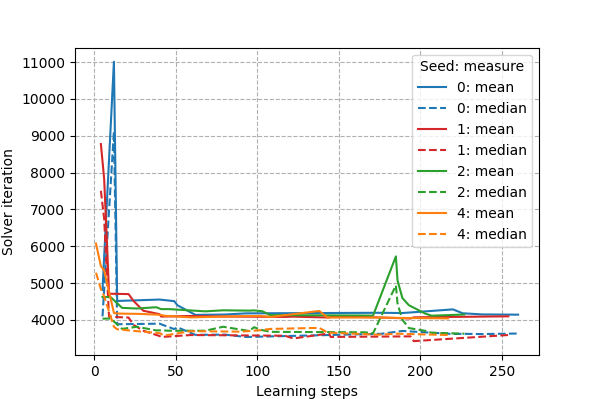
\includegraphics[width=1\textwidth]{plots/large_learning_curve_zoom.png}
        \caption{Learning curves for from the learning of the larger systems, where the colour of the curve corresponds to the different seeds.\\\\}
        \label{fig: large learning curves}
    \end{minipage}
    \begin{minipage}{.02\textwidth}
        
    \end{minipage}
    \begin{minipage}{.49\textwidth}
        \center
        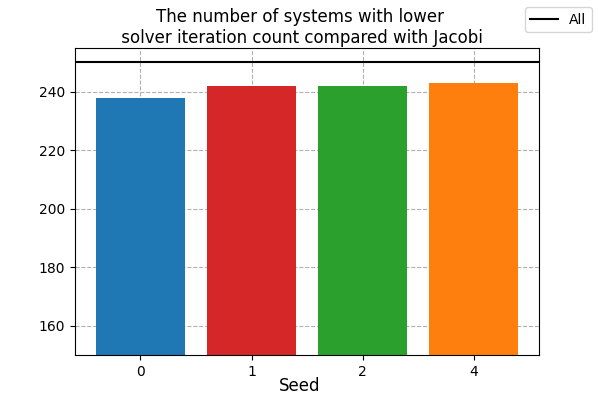
\includegraphics[width=1\textwidth]{plots/large_BvJ.png}
        \caption{Graph showing how many individual systems that has a lower solver iteration count with the learned preconditioners compared with its Jacobi preconditioned counterpart from the different seeds. With an y-axis offset of 150.}
        \label{fig: large BvJ}
    \end{minipage}
\end{figure}

\begin{figure}[H]
    \center
    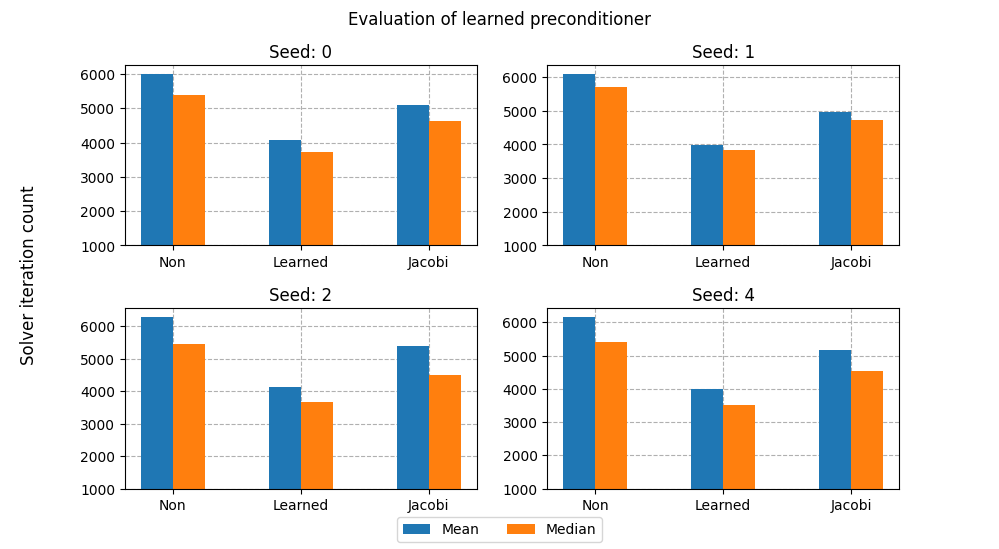
\includegraphics[width=0.9\textwidth]{plots/large_test_measure.png}
    \caption{Mean (blue) and median (orange) solver iteration counts from the evaluation of the learned preconditioners, with unpreconditioned and Jacobi preconditioning for comparison, with a plot for each of the seeds.}
    \label{fig: large test measure}
\end{figure}
    

From learning curves in figure \ref{fig: large learning curves} we can see what we have seen many times in the previous tests. That is the mean and median solve iteration counts decrease during the learning quickly and therefore plateaus. For example for seed 1, red curve, starts with a mean solver iteration count 8773.2 and decreases to a count a bit above 4000, and similar curves for the other seeds.

In the evaluation of the learned preconditioners, we can see that the preconditioners decreases the mean and median solver iteration count by approximately 2000 iterations compared to using no preconditioner and 1000 compared with Jacobi preconditioning, figure \ref{fig: large test measure}. For the individual comparisons in figure \ref{fig: large BvJ} that around 240 system with the learned preconditioner have a lower solver iteration count compared with using Jacobi preconditioning. Meaning it is fair to say that the algorithm has learned a good preconditioner for the larger system sizes for all four seeds.


